\subsection{Calculation of input water discharge}
The simulator transfers water in hydrographic channel from upstream RS to discharge system RS. At each node, upper hydrograms are cumulated and propagated to downstream RS.

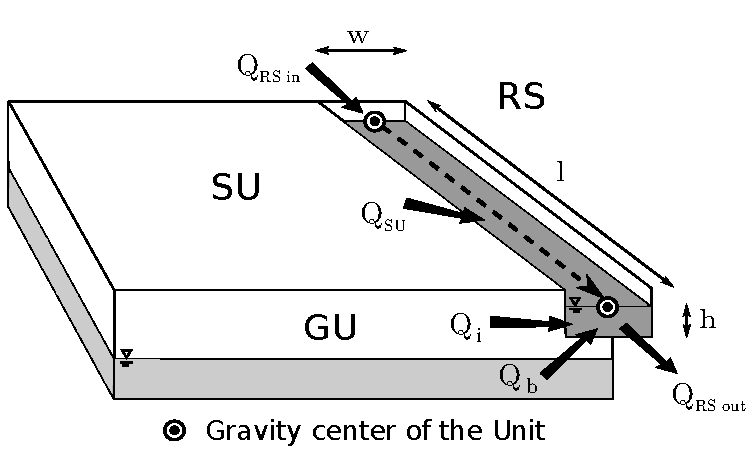
\includegraphics[width=8cm]{doc/common/Schema_GU_RS_SU_Hayami_RS.pdf}

The first step consists in computing the input discharge at the inlet of the ditch. This value is composed with discharge from potential connected RS or SU and subsurface and aquifer drainage flow if the model previously produces these variables. The equation is the following :

\begin{equation}
\label{InputDischarge}
Q_{in} = \sum_{RS_{Up}} Q_{RS} + \sum_{SU_{Up}} (Q_{SU} + Q_i) + \sum_{GU_{Up}} Q_b
\end{equation}


where $Q_in$ is the input water discharge at the inlet of the RS ($m\up3/s$), $Q_{RS}$ is the discharge produced by the upper connected RS, $Q_{SU}$ is the discharge from the upper SU, $Q_b$ is the baseflow discharge from connected GU ($m\up3/s$), and $Q_i$ is the interflow discharge ($m\up3/s$).\\


\subsection{Propagation using Hayami kernel}
Then, the input water discharge previously calculated is propagated between the gravity center of the main SU and the downstream unit. The propagation is done using the diffusive wave model \cite{Moussa1997} :

\begin{equation}
\frac{\delta Q}{\delta t} = -C \times \frac{\delta Q}{\delta x} + D \delta \frac{\delta \up2 Q}{\delta x\up2}
\end{equation}




In the particular case where wave celerity and diffusivity are constant, the diffusive wave equation can be resolved using an analytical solution \cite{Moussa1996}. The water output discharge is calculated using the following equation :

\begin{equation}
\label{HayamiConvolution}
Q_{RS}(t) = Q_{in}(t) * K(t)
\end{equation}




where $Q_{RS}$ is the produced output water discharge ($m\up3/s$), $Q_{in}$ is the input water discharge on RS ($m\up3/s$) calculated in the equation \ref{InputDischarge}, $*$ is the convolution product, and $K(t)$ is the ``Hayami kernel'' function expressed as :

\begin{equation}
K(t) = \frac{L}{2 \times (\pi D)^{\frac{1}{2}}} \times \frac{\text{exp}^{\frac{CL}{4D} \times \left(2-\frac{L}{Ct}- \frac{Ct}{L} \right) } }{t^{\frac{3}{2}}}
\end{equation}




where $L$ is the length of RS ($m$), $D$ is the wave diffusivity ($m\up2/s$), and $C$ is the wave celerity ($m/s$).\\

To resolved the equation \ref{HayamiConvolution}, the simulator temporarily sweeps the Hayami kernel. $\tau$ is a convolution time with $\delta \tau$ wich is equal to the simulation time step. This operation can be schematized as following :

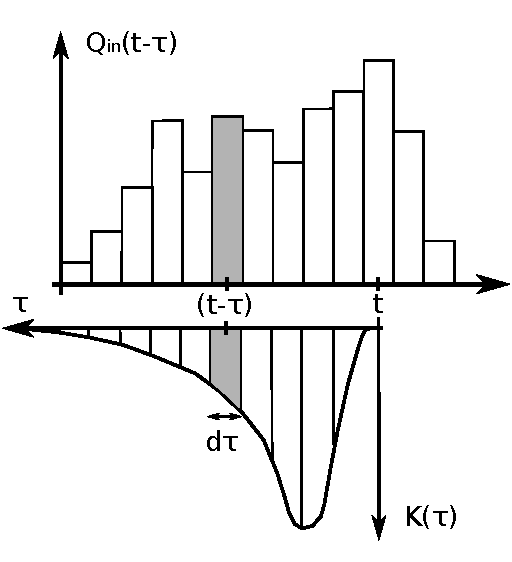
\includegraphics[width=8cm]{doc/common/Convolution_HayamiRS.pdf}

The $K(t)$ function of Hayami Kernel is defined on [0 +$\infty$]. However, the kernel covolution cannot be done up to the infinity. $MaxSteps$ parameter ($-$) defines the number of time step and, consequently, the limit duration $MaxSteps . \Delta t$. It should be adapted according to the kernel shape and the simulation time step in the way to minimise the kernel truncation. The higher this parameter is, the better the definition of Hayami kernel is. Moreover, the smaller the simulation time step is, the better the Hayami kernel resolution is. The optimal way to parametrise the model for a given simulation time step is to start from a height value of $MaxSteps$ and then dicreases it while no change on results.\\

The two main parameters $C$ and $D$ of the diffusive model could be related to the slope and the rugosity of the surface unit using Manning-Strickler relation.

\begin{equation}
C=C_u \times \sqrt{\frac{\beta}{\beta_m}}\times \frac{n_m}{n} \ \ \ \ \ et \ \ \ \ \ D=D_u\times \frac{\beta}{\beta_m} \times \frac{n_m}{n}
\end{equation}


where $C_u$ is the mean wave celerity ($m/s$), $\beta$ is the slope of the RS on which the calculation is done ($m/m$), $\beta_m$ is the mean slope of RSs ($m/m$), $n$ is the rugosity coefficient of the RS ($s/m\up{1/3}$), $n_m$ is the mean rugosity coefficient of RSs ($s/m\up{1/3}$) and $D_u$ is the mean wave diffusivity ($m\up2/s$). This calculation is done once at the beginning of the simulation.\\

Diffusivity and celerity define the shape of Hayami unit hydrogram as :

\begin{equation}
w = \frac{L}{D} \ \ \ \ \ z = \frac{C.L}{4.D}
\end{equation}



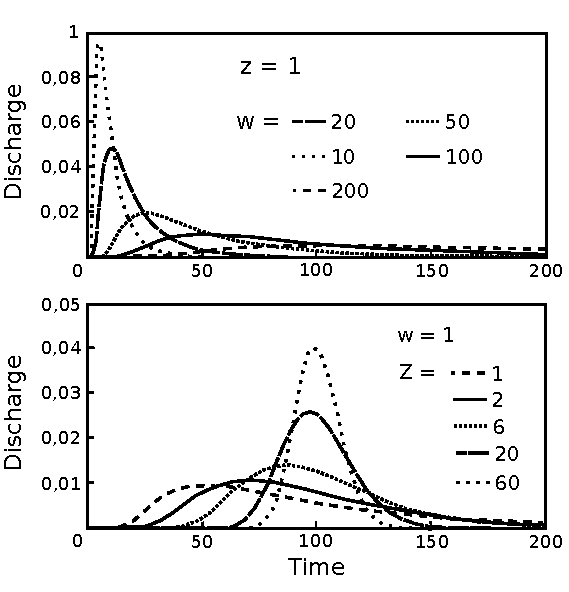
\includegraphics[width=8cm]{doc/common/Graphique_noyau_Hayami.pdf}

Examples of use and parametrization of this model are available in the thesis of Chahinian \cite{Chahinian2004} and a paper of Moussa and al. \cite{Moussa2002}.


\subsection{Discharge - Height conversion}
Then, the simulator converts the previous calculated discharge to water height in the reach segment. This convertion is done using the Manning-Strickler equation which links height and discharge for a rectangular ditch section :

\begin{equation}
Q_{RS} = \frac{1}{n} \times \sqrt{\beta} \times R^\frac{2}{3} \times l \times h \ \ \ \ \text{with} \ \ \ \ R = \frac{l \times h}{l + 2h}
\end{equation}




where $n$ is the rugosity coefficient of RS ($s/m\up{1/3}$), $\beta$ is the slope of RS ($m/m$), $R$ is the hydraulic radius of the ditch ($m$) considered as a rectangular section, $l$ is the width of RS ($m$), and $h$ is the water height in the reach segment ($m$) corresponding to discharge.\\

The simulator compute height-discharge relation using the previous equation, 
once for each RS at the begining of the simulation. Then, the obtained curve is 
used to determine for each time step the water height corresponding to the 
calculated output discharge $Q_{RS}$. The calibration curve of the RS is 
computed with a ``height step'' given by the $Calib Step$ parameter (in $m$). 
The smaller this parameter is, the more accurate the calculated water height 
is. This relation is calculated up to a maximum height which is the RS height 
$H$ plus the $RS buffer$ parameter (in $m$). Up to this value, the simulator displays a warning which indicated that the RS water height is out of range.\\

